\chapter{绪论}

\section{研究背景与意义}
    随着微电子技术的发展,硬件计算水平已经达到了前所未有的高度,这促使九十年代一度被人忽视的神经网络算法得到飞速发展,尤其是在图像识别领域,神经网络越来越受到人们的重视。
    神经网络具有自适应学习能力,也可以根据不同的需求更改网络的复杂度,同时对噪声不太敏感,相比与传统的识别方法,神经网络算法具备更高的鲁棒性。

    时下,由于神经网络算法中存在这海量的参数、复杂的计算过程,因此传统的方法是通过CPU + GPU/TPU架构进行模型的训练工作,这种方法利用了GPU多核、并行计算的特性取得了十分显著的效果。
    但这种架构需要数百瓦的功率支持,同时需要较大的物理空间放置设备,缺乏灵活性,无法满足IoT领域的要求。

    针对IoT领域对续航、灵活性的需求,异构计算芯片成为了极佳的解决方案。当前,一些基于异构处理器的边缘计算方案已经取得了令人瞩目的成绩,例如Google近期推出的搭载了TPU的单板计算机——Coral。
    \begin{figure}
        \centering
        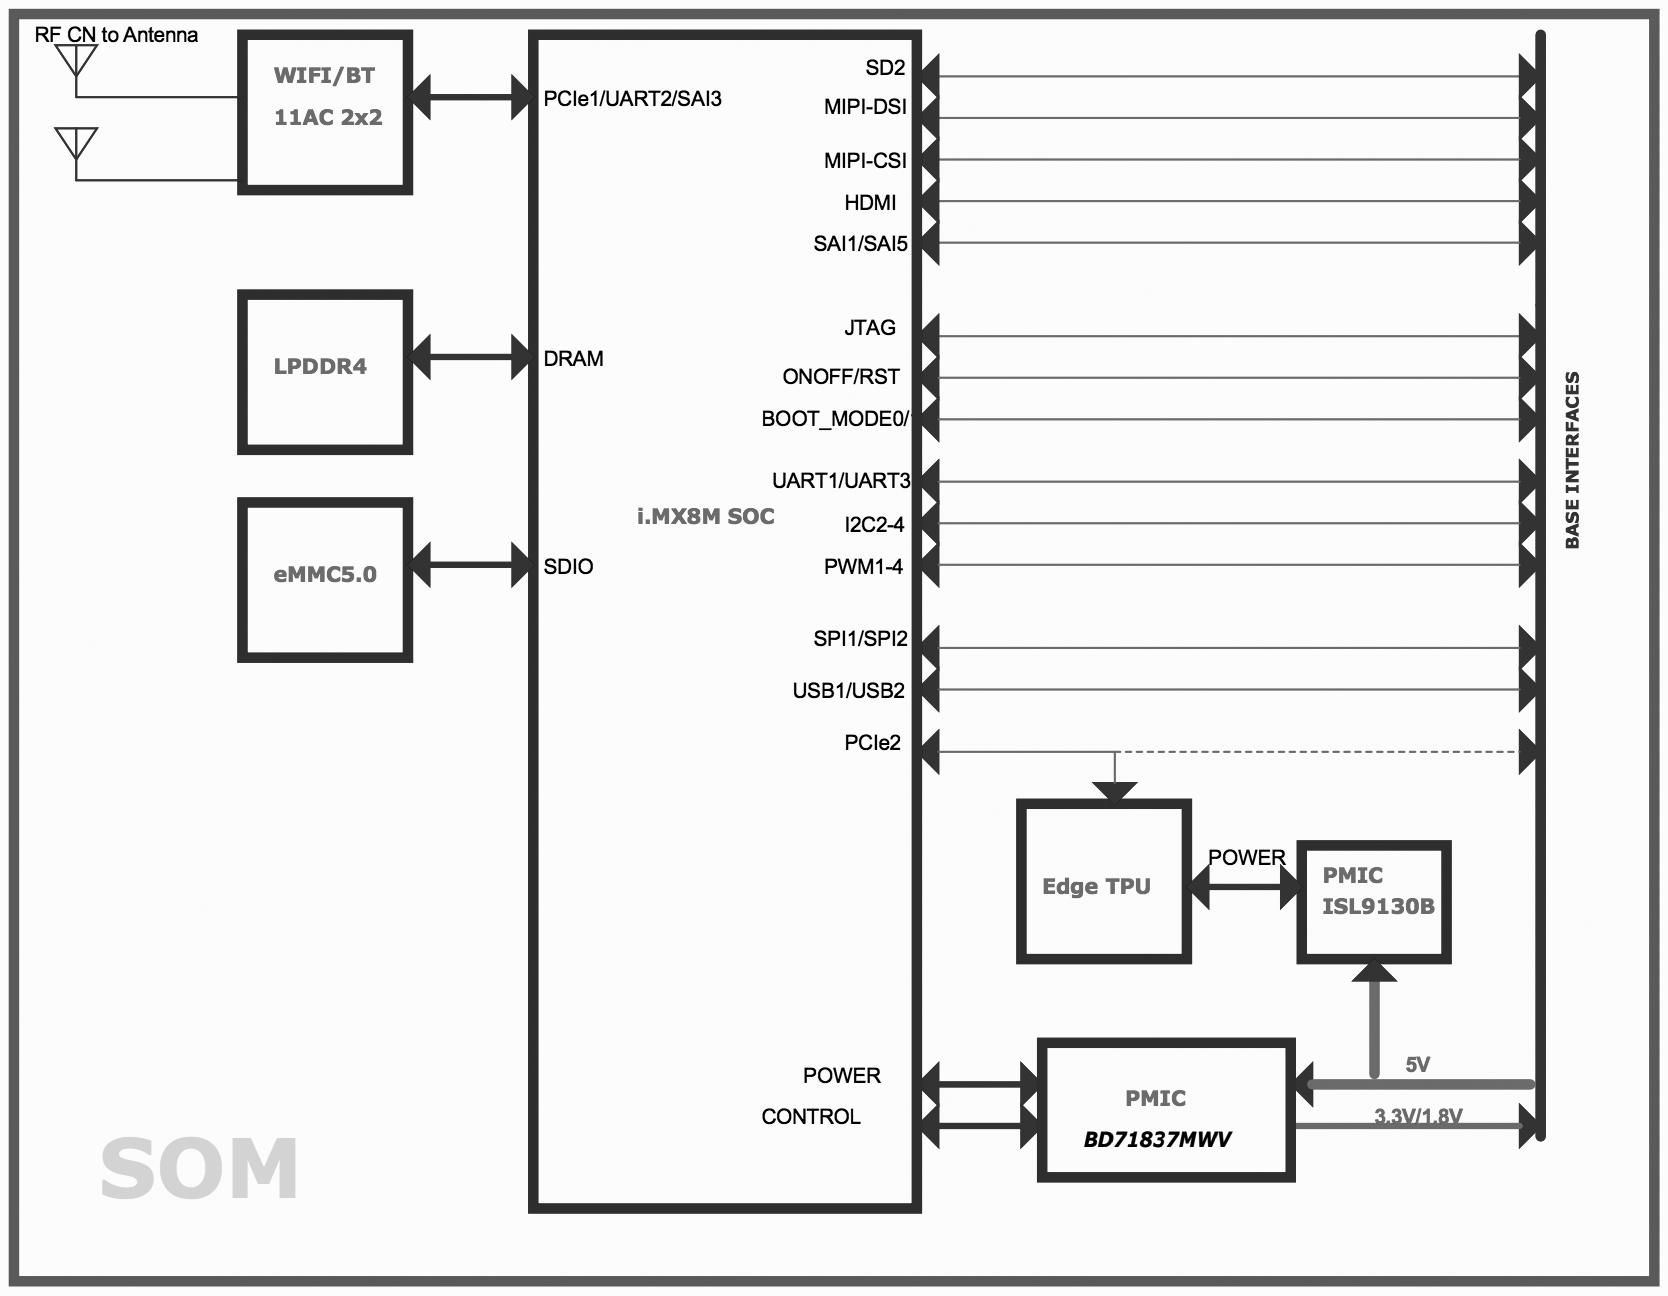
\includegraphics[scale=0.2]{../pdf/coral.png}
        \caption{Coral开发板SoM架构图}
        \label{coral}
    \end{figure}
    从图\ref{coral}可以看出,Coral架构中采用了NXP的i.MX8 SoC与Google研发的TPU模块通过PCIe2总线进行通信,二者组成异构计算平台,计算性能远超树莓派。

    本文通过研究Eyeriss架构,针对IoT领域,综合考虑算力、能耗、成本,开发一套基于异构处理器的用于图像识别的CNN计算加速系统。

\section{国内外发展现状}
    从 2015 年开始,AI 芯片的相关研发逐渐成为学术界和工业界研发的热点。到目前为止,在云端和终端已经有很多专门为 AI 应用设计的芯片和硬件系统。
    针对需求,目标应用可以划分为“ 训练”或者“推断”,目前在边缘 / 嵌入设备中以推断应用为主,
    训练的需求还不是很明确。有些高性能的边缘设备虽然也会进行训练,但从硬件本身来说,它们更类似于云端设备。
    未来的边缘和嵌入设备可能都需要具备一定的学习能力,以支持在线学习功能。

    文献[2]作者考虑到性能、功耗、灵活性,认为在嵌入式领域基于FPGA的DNN加速器是较为明智的选择。但是FPGA开发相对于软件开发更加困难,因此其提出了一种名为FP-DNN (FieldProgrammable DNN)的端到端框架。该框架使用TensorFlow描述的DNN作为输入,然后自动生成RTL-HLS混合的模板。文献[3]同样基于高层次方法的设计,方法与文献[2]大同小异。其实验数据表明性能是CPU的17.65倍。
    以上两篇文献设计方法是从高级语言框架(Tensorflow、Caffe等)入手,经过开发的编译器或者HLS技术映射到FPGA中,这种方法具有硬件开发周期短、工作量少的优势,但由于编译器和HLS技术的不完善,从高级语言编译出的RTL电路缺乏对硬件潜在的并行特性的开发,无法完全发挥出硬件电路的优势。
    文献[4]给出了另一种FPGA实现DNN的途径。其构造了一个DLAU (Deep Learning Accelerator Unit),该单元是一个可扩展DNN计算加速器,内含三级流水线,极大提高了数据吞吐量,其测试数据表明此方案比Intel双核处理器加速了36.1倍。这种设计方法更加符合硬件工程师思维,同时性能更加优异,但是其开发难度较大,且需要自行构造一些自动化工具来进行DNN系统配置。文献[5]给出了一种玻尔兹曼机的高性能FPGA实现,玻尔兹曼机可以理解为神经网络中的一个神经单元,文中描述软件实现的神经网络其复杂度是O(n2)级别,因此其无法提供非学术的性能和扩展性。文献作者充分利用了硬件潜在的并行特性构造的受限玻尔兹曼机将复杂度降低为O(n)级别,同时仅仅需要O(n)级别的资源。根据其在Xilinx Virtex II-Pro XC2VP70 上的测试,其可运行在100MHz频率,比2.8GHz的Intel处理器加速了35倍。
    现如今AI芯片的开发尚未出现标准的方法学,两种主流方案,其一是基于当前发展成熟的深度学习框架,将使用高级语言编写的DNN系统翻译成RTL电路,该方案开发周期短,且开发较为容易,但受限于编译器的缺陷,没有完全发挥硬件电路的特性;其二是构造一可扩展的单个神经元并配合自动化脚本,生成所需的DNN系统,该方案开发难度较大,但可以充分发挥硬件的特性,性能更加优秀。

\section{论文的主要研究内容及意义}
    本文主要基于文献[X]的思想,结合近几年发展起来的敏捷型HDL开发语言——Chisel,编写一款PE阵列生成器,可配置阵列大小、计算位宽、FIFO深度来满足不同神经网络的需要,
    结合异构处理器,完成对CNN的加速推断。

    同时,本课题对比了传统数字电路开发方法与敏捷型数字电路开发方法的优劣,探讨了基于敏捷型开发方法的流程。在新方法的框架下完成CNN加速系统加速器部分的开发。并通过Xilinx Vivado集成开发环境,完成系统的性能评估。
    运行一量化的手写数字识别网络,完成对系统的逻辑功能验证。

    本课题一方面可以帮助数字电路开发人员直观的比较传统Verilog与新型Chisel两种HDL语言的区别,方便对新技术有个全面的认识,另一方面构造的PE阵列生成器,可以十分方便的生成所需的规模,加速对不同AI应用场景加速系统的开发流程。

\section{论文章节安排}
    结合国内外发展现状,利用Chisel语言的特性,确定了基于异构处理器图像识别系统的需求设计,本文工作安排如下:

    第一章:绪论。本章简单介绍了当下国内外针对AI推断加速的主要成果以及主要研究内容和意义

    第二章:开发工具及相关技术介绍。本章首先简单介绍了基于JVM的Scala语言及其特性,随后重点介绍了基于Scala语言开发的Chisel语言的特性、使用方法、与Verilog的区别、开发流程。
    同时介绍了Verilator——一个开源、高性能的Verilog仿真工具。其次介绍了当前主流的两种异构处理器架构或平台,RISC-V和ZYNQ。最后介绍了神经网络在图像识别领域的典型应用和案例。

    第三章:系统功能需求分析与系统架构设计。本章首先介绍了传统架构和异构的优劣势,随后针对第二章介绍了两个异构平台设计了两种针对图像识别领域的CNN加速系统,其次简单描述了一下采用HLS与HDL两种开发的优劣,其中引出了敏捷型开发思想。
    最后详细介绍了在异构平台上计算任务的划分方法,以及基于行静止思想的卷积计算方法。
    
    第四章:硬件模块介绍。本章详细介绍了每一个PE阵列中使用的模块的引脚、功能、内部结构设计。最后详细介绍了充分发挥Chisel特性的PE阵列生成器的代码结构,以及其可配置参数的功能

    第五章:功能仿真结果。本章主要介绍了单个PE的仿真波形,详细介绍了每个阶段的关键信号以及逻辑行为,其次对一个6×7PE阵列的4D卷积计算波形图,并给出了综合实现之后的资源使用报告和时序报告。

    第六章:板级测试结果。本章基于PYNQ平台,集成开发的PE阵列开发了一个用于测试的板级系统,展示了基于一个int8量化的MNIST网络的实际运行结果。

% \subsection{二级节标题}

% \subsubsection{三级节标题}

% \paragraph{四级节标题}

% \subparagraph{五级节标题}

% \section{脚注}

% Lorem ipsum dolor sit amet, consectetur adipiscing elit, sed do eiusmod tempor
% incididunt ut labore et dolore magna aliqua. Ut enim ad minim veniam, quis
% nostrud exercitation ullamco laboris nisi ut aliquip ex ea commodo consequat.
% Duis aute irure dolor in reprehenderit in voluptate velit esse cillum dolore eu
% fugiat nulla pariatur. Excepteur sint occaecat cupidatat non proident, sunt in
% culpa qui officia deserunt mollit anim id est laborum.
% \footnote{This is a long long long long long long long long long long long long
% long long long long long long long long long long footnote.}
